\section{Atome und Moleküle - Grundlagen eines Festkörpers}

\subsection{Grundaufbau eines Atoms}
Ein Atom besteht aus einem Kern, der Protonen (positiv geladen) und Neutronen (ungeladen) enthält, und einer den Kern umschliessenden Wolke aus Elektronen (negativ geladen).\\
Ein Atomkern wird durch die \textbf{Ordnungszahl Z} beschrieben.\\
\\
\textbf{Coulombpotential ($\varepsilon_0 = 8.85\cdot 10^{-12}\frac{\mathrm{As}}{\mathrm{Vm}}$):}
\begin{center}
	$\begin{matrix}
		\displaystyle U_{\text{Coulomb}}\left(\vec{r}, Q\right) = \frac{1}{4\pi\varepsilon_0}\cdot \frac{Q}{\mid\vec{R} - \vec{r}\mid}
	\end{matrix}$\qquad\qquad
	\begin{tabular}{ll}
		Q & Ladung\\
		$\vec{R}$ & Ort Ladung\\
		$\vec{r}$ & beliebiger Ort\\
	\end{tabular}
\end{center}

\textbf{Potentielle Energie eines geladenen Teilchens q am Ort $\vec{r}$ :}

$$\displaystyle E_{\text{Coulomb}}(\vec{r}, q) = U_{\text{Coulomb}} \cdot q = \frac{1}{4\pi\varepsilon_0}\cdot \frac{Qq}{\mid\vec{R} - \vec{r}\mid}$$ %TODO: Richtig?

\subsection{Bohr'sches Atommodell}
Im Bohr'schen Atommodell geht man davon aus, dass Elektronen den Kern umkreisen.\\
Der Bahndrehimpuls \textbf{L} der Elektronen auf ihren möglichen Trajektorien ist gequantelt :
\begin{center}
	$\begin{matrix}
		L = n \cdot \hbar  = n\cdot\frac{h}{2\pi}  
	\end{matrix}$
	\begin{tabular}{ll}
		$n \in \mathbb{N}$, Schalen, Hauptquantenzahl\\
		$h = 6.626\cdot10^{-34}\text{Js} =$
		Planck’sche Wirkungsquantum\\
	\end{tabular}
\end{center}

\subsubsection{Bohr'scher Radius}
Der Bohr’sche Radius ist definiert als der kleinste Radius, welcher ein Elektron im
Wasserstoff-Atom ($n$ = 1) annehmen kann;

$$r_{\text{Bohr}} = 4\pi\varepsilon_0\cdot\frac{n^2 \hbar^{2}}{m_{e}e^{2}} = 5.3\cdot10^{-11}\text{m}$$

\subsubsection{Ionisierungsenergie und Viralsatz}
Als sogenannte \textbf{Ionisierungsenergie} wird diejenige Energie bezeichnet, die man aufbringen
muss, um ein Elektron vom Kern zu entfernen;

$$E_{tot} = E_{kin} + E_{pot} = \frac{1}{2}m_{e}v^{2} + E_{Coulomb}$$

\textbf{Viralsatz :}
$$\langle E_{tot}\rangle = \langle E_{kin}\rangle + \langle E_{pot}\rangle  \text{\qquad und \qquad} \langle E_{kin}\rangle = - \frac{1}{2}\langle E_{pot}\rangle$$

\subsubsection{Formula di Rydberg ($\Delta E$ per i salti elettronici)}
Questa formula permette di calcolare la differenza di energia associata al 'salto' di un elettrone da un livello energetico di partenza a uno di arrivo all'interno di un atomo idrogenoide

\begin{minipage}{0.35\columnwidth}
	$$\Delta E = -Z^2 \cdot E_I \cdot \left(\frac{1}{n_j^2} - \frac{1}{n_i^2}\right)$$
\end{minipage}
\hfill
\begin{minipage}{0.63\columnwidth}
	\begin{itemize}
    \item $Z$: Numero atomico dell'elemento
    \item $E_I$: Energia di ionizzazione (idrogeno $= 13.6 \text{ eV}$).
    \item $n_j$: Numero quantico del livello di partenza.
    \item $n_i$: Numero quantico del livello di arrivo.
\end{itemize}
\end{minipage}

\subsection{Das Schalenmodell, mit Unterschalen und Orbitalen}
Die Schale mit \textbf{Hauptquantenzahl n} hat \textbf{n Unterschalen}, welche durch die \textbf{Bahndrehimpulsquantenzahl l} beschrieben werden.

\begin{tabular}{ll}
	s,p,d,f,... & Bahndrehimpulsquantenzahl\\
	K,L,M,N,... & Hauptquantenzahlen 1,2,3,4,...\\
\end{tabular}


\begin{minipage}{0.48\linewidth}
	Maximum possible number of electrons in the shells and subshells of an atom\vspace{1em}

	\begin{tabular}{cccccc}
		& & \multicolumn{4}{c}{\textbf{Subshell}} \\ \cline{3-6} 
		& & $\ell = 0$ & $\mathbf{1}$ & $\mathbf{2}$ & $\mathbf{3}$ \\
		$n$ & \textbf{Shell} & $s$ & $p$ & $d$ & $f$ \\ \hline
		1 & $K$ & 2 & & & \\
		2 & $L$ & 2 & 6 & & \\
		3 & $M$ & 2 & 6 & 10 & \\
		4 & $N$ & 2 & 6 & 10 & 14 \\ \hline
	\end{tabular}
\end{minipage}
\hfill
\begin{minipage}{0.48\linewidth}
	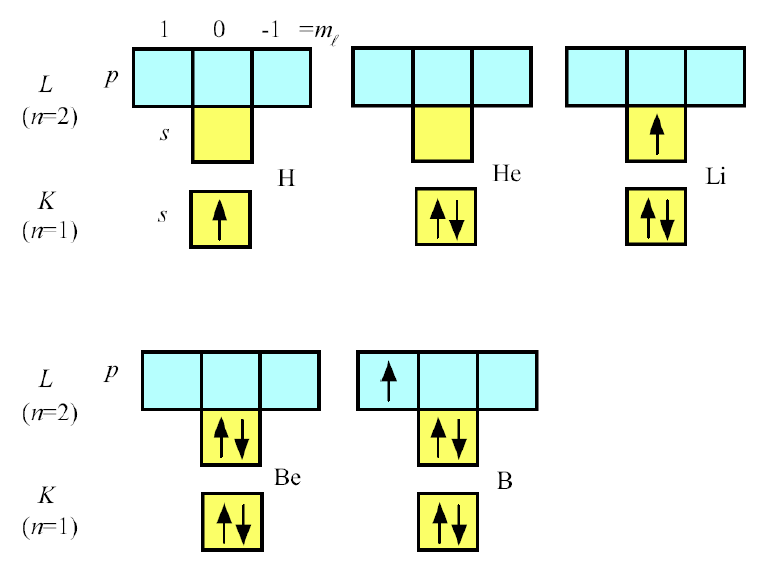
\includegraphics[width=\linewidth]{Bilder/Kaestchen}
\end{minipage}

\subsubsection{Pauli-Prinzip}\label{chap:pauli}
Keine zwei Elektronen in einem System (z.B. in einem Atom) können dieselben
Quantenzahlen haben. Für die Bahndrehimpulsquantenzahl $l$ gibt es 
$$\boxed{2l + 1}$$
Kästchen (Orbitale), welchen
man wiederum ganzzahlige, magnetische Quantenzahlen zuordnen kann. Folgende Werte werden
zugewiesen: $m_{l} \in \{-l,-l + 1, ..., -1,0,1,...,l -1,l\}$.\\

\textbf{Per convenzione le Kästchen vengono riempite prima con spin verso l'alto $\uparrow$\vspace{1em}}

\begin{minipage}{0.48\linewidth}
	Um das Pauli-Prinzip nicht zu verletzen gibt es noch die vierte Quantenzahl, die \textbf{Spin-Quantenzahl}(kurz Spin);

	$m_s \in \left\{-\frac{1}{2}, +\frac{1}{2} \right\}$
\end{minipage}
\hfill
\begin{minipage}{0.48\linewidth}
	$\Rightarrow$
	\begin{tabular}{ll}
		Hauptquantenzahl & $n$\\
		Bahndrehimpulsquantenzahl & $l$\\
		magnetische Quantenzahl & $m_l$\\
		Spin & $m_s$\\
	\end{tabular}
\end{minipage}

\subsubsection{Hund'sche Regel}
\begin{minipage}{0.5\linewidth}
	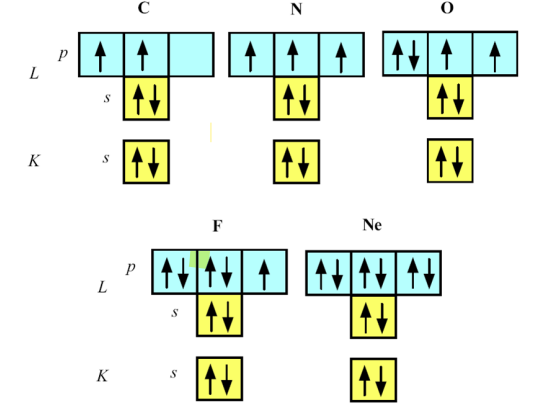
\includegraphics[width=0.9\linewidth]{Bilder/Füllung_Schalen}
\end{minipage}
\begin{minipage}{0.5\linewidth}
	Elektronen mit gleicher Hauptquantenzahl $n$ und Bahndrehimpulsquantenzahl $l$ haben bevorzugterweise denselben Spin $m_s$

	Füllung bei teilgefüllten Unterschalen gemäss der Hund’schen Regel:
\end{minipage}

\subsection{Bindungstypen von Molekülen}
\subsubsection{Grund-Prinzip von Bindungen zwischen Atomen}
	Damit Atome eine Bindung eingehen, muss folgendes Kräftegleichgewicht herrschen:

	$F_{\text{Bindung}} = F_{\text{anziehend}} + F_{\text{abstossend}}$

	Alternativ kann man die Bindung auch im Potential anschauen, welches auch als Lennard-Jones-Potential bekannt ist. 
	Die potentielle Energie aufgrund des Lennard-Jones Potentials lautet wie folgt:

	\begin{minipage}{0.6\linewidth}
		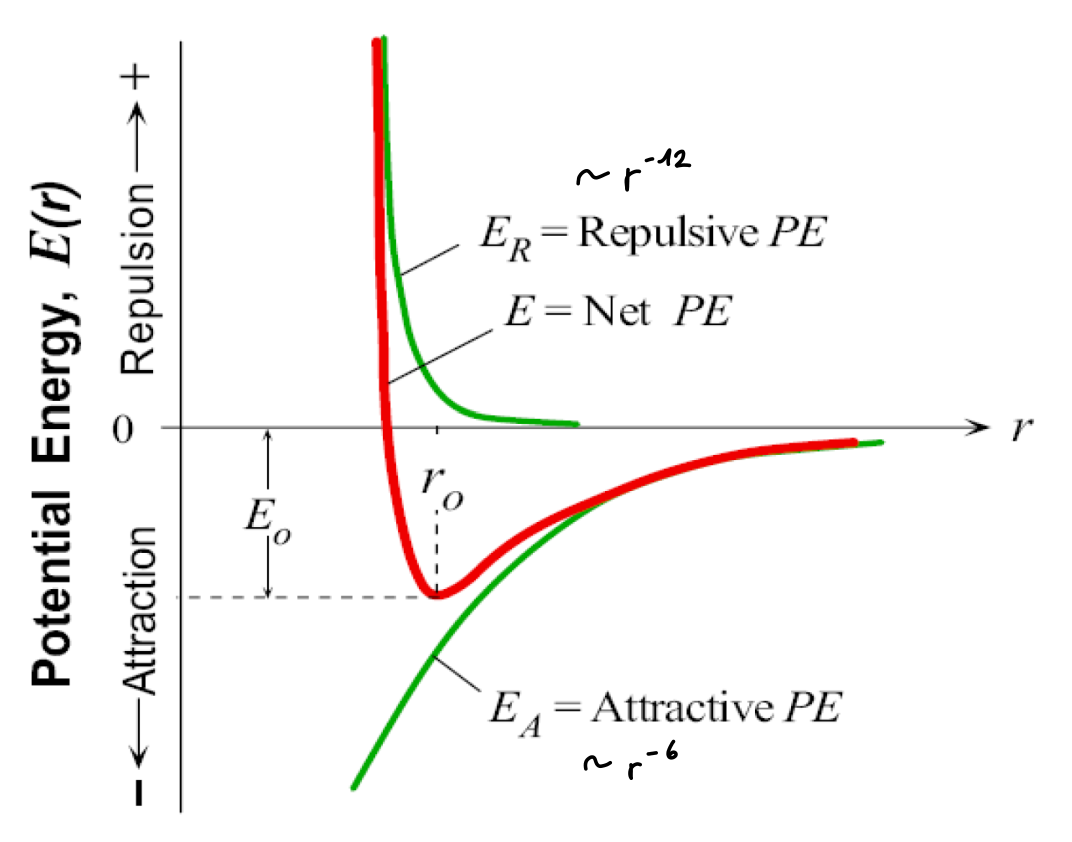
\includegraphics[width=0.9\linewidth]{Bilder/Lennard_Jones}
	\end{minipage}
	\hfill
	\begin{minipage}{0.38\linewidth}
		$$E_{\text{Lennard-Jones}} = -A\frac{1}{r^6} + B\frac{1}{r^{12}}$$\vspace{1em}

		wobei $A$ und $B$ Vorfaktoren sind und vom jeweiligen Element abhängen
	\end{minipage}

\subsubsection{Kovalente Bindung}
	Bei der kovalenten Bindung teilen sich 2 Atome die Valenzelektronen für eine volle Schale

	\begin{minipage}{0.55\linewidth}
		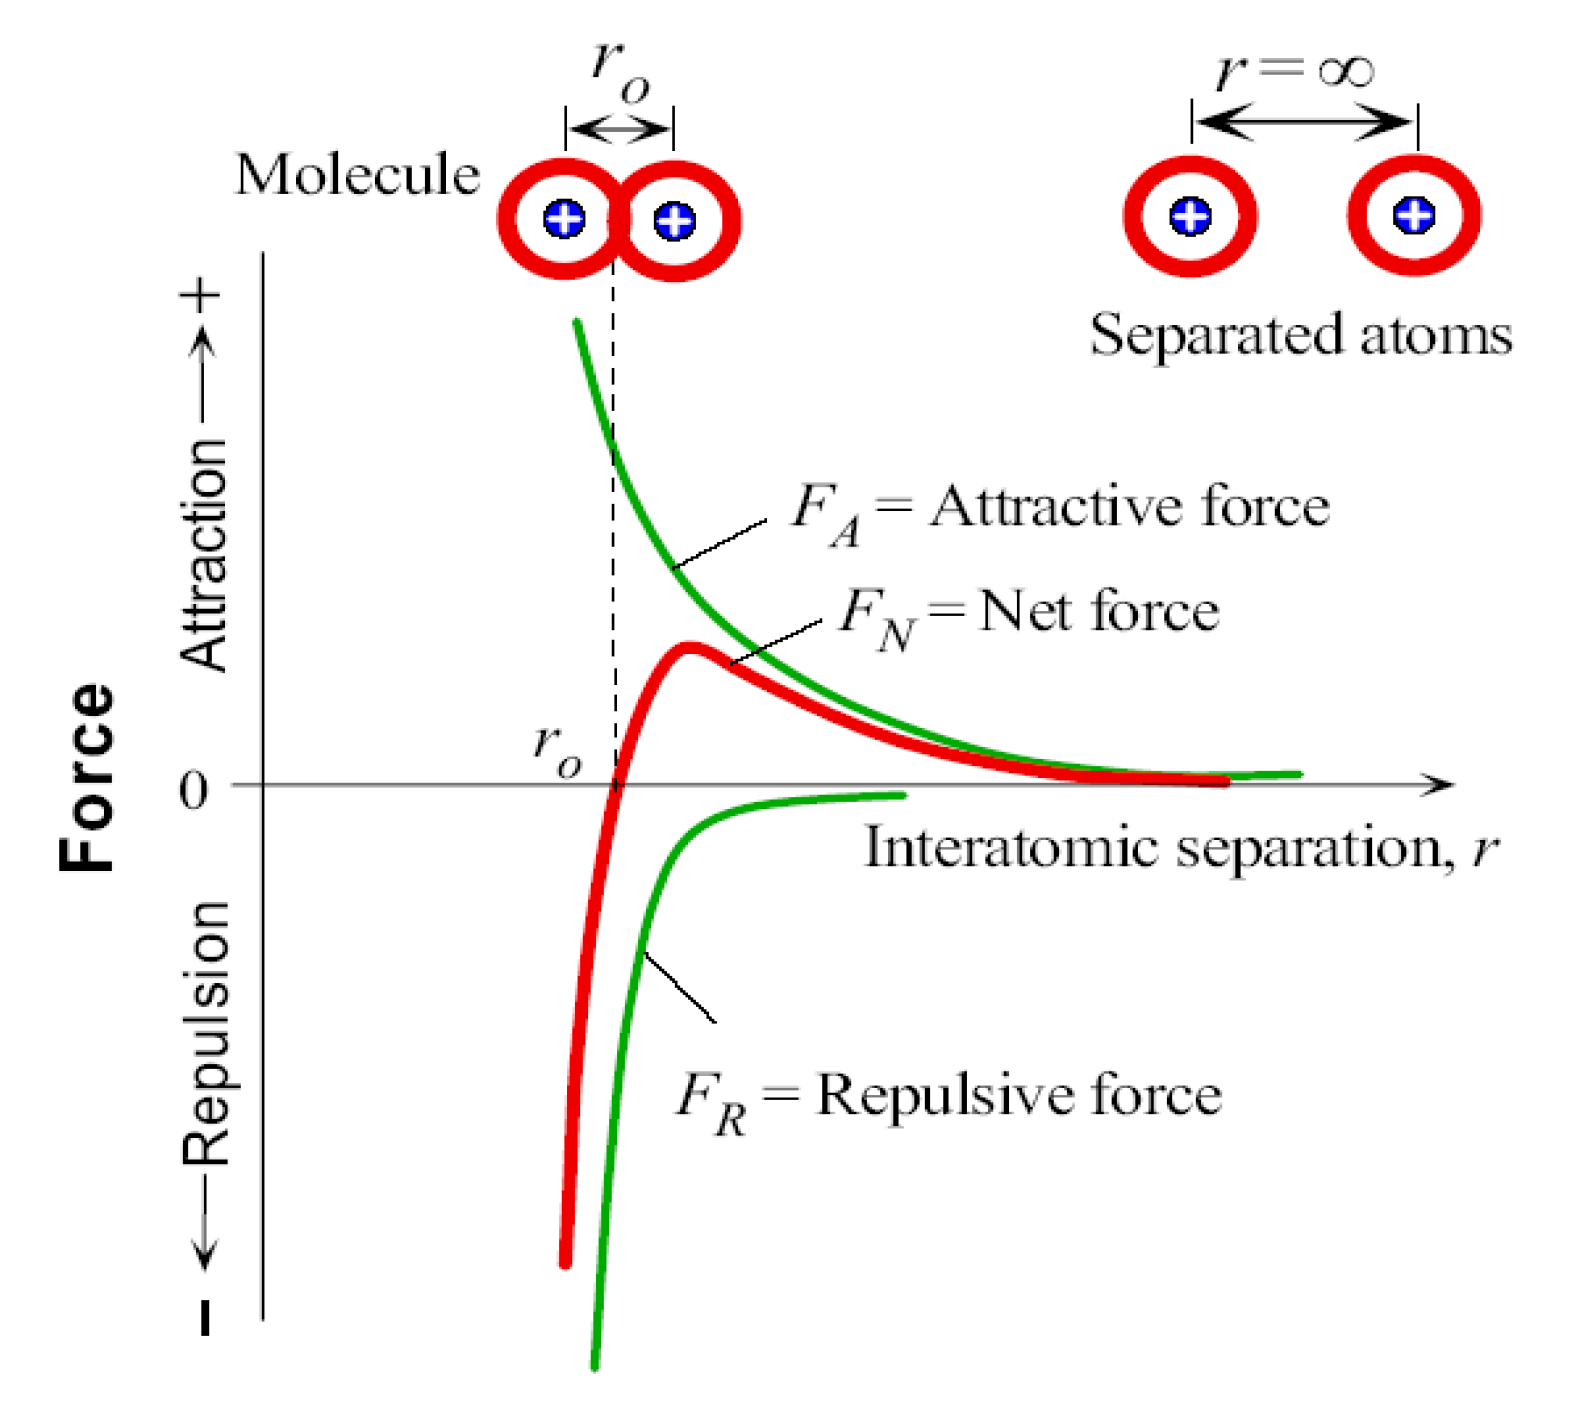
\includegraphics[width=\linewidth]{Bilder/Kovalent_1}
	\end{minipage}
	\begin{minipage}{0.45\linewidth}
		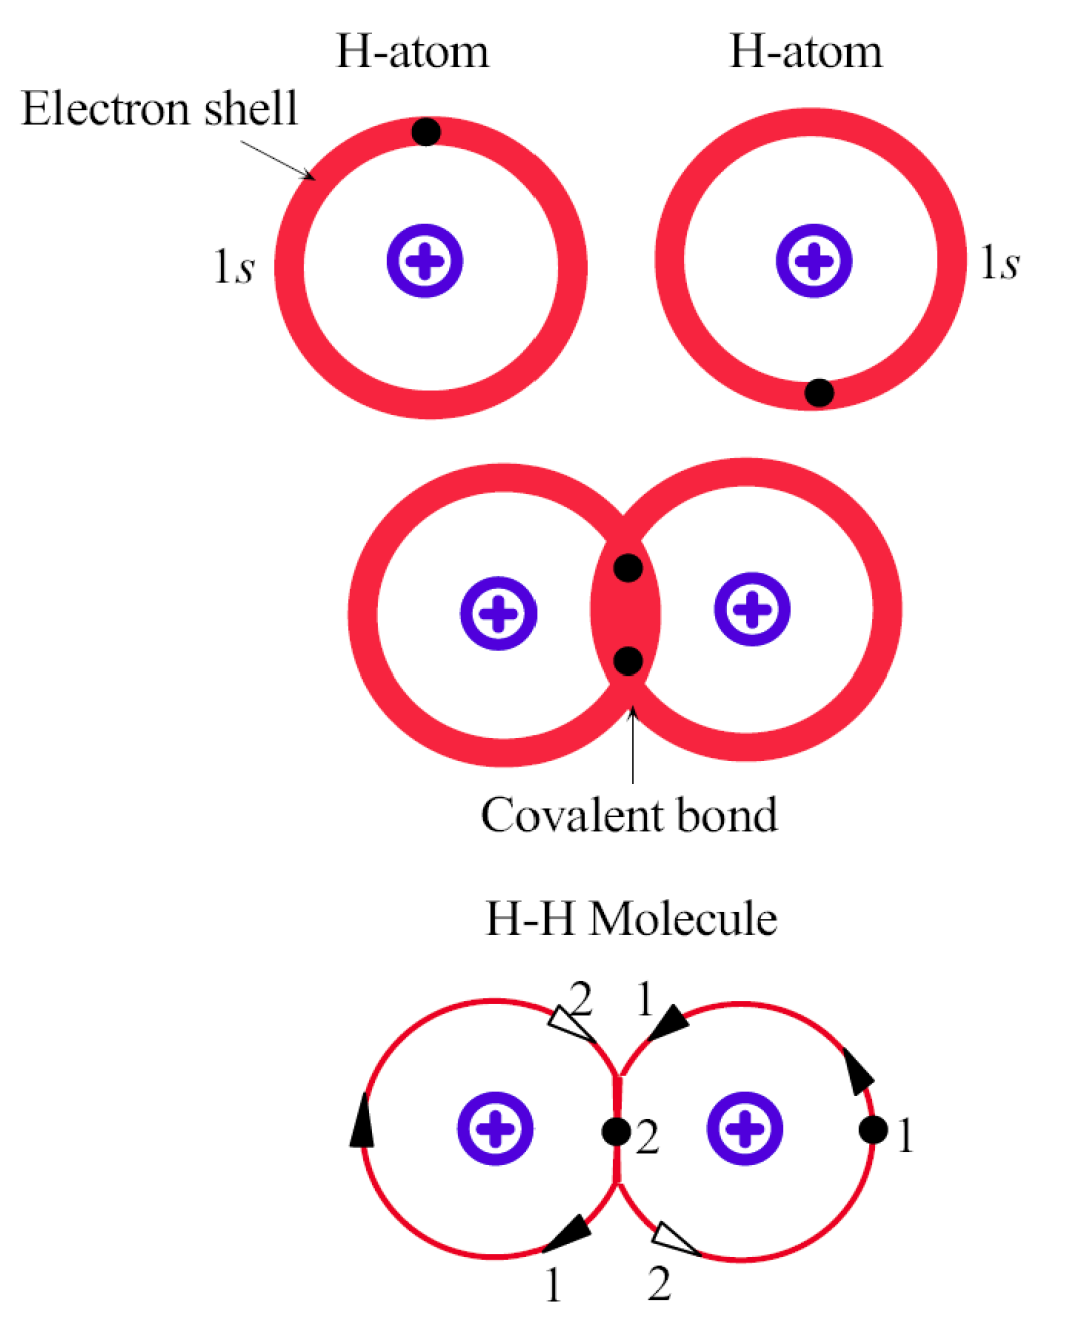
\includegraphics[width=0.9\linewidth]{Bilder/Kovalent_2}
	\end{minipage}

\subsubsection{Metallische Bindung}
	\begin{minipage}{0.45\linewidth}
		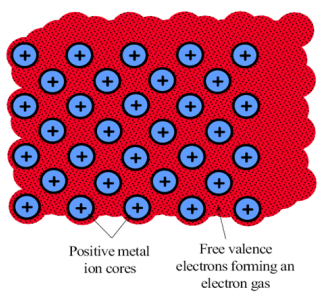
\includegraphics[width=0.9\linewidth]{Bilder/Metallbindung}
	\end{minipage}
	\hfill
	\begin{minipage}{0.53\linewidth}
		\begin{itemize}
			\item Typischerweise Elemente mit \textbf{wenig Valenzelektronen} $\to$ tendieren zur Elektronen-Abgabe
			\item Abschirmung durch sog. \textbf{Elektronengas} $\to$ Elektronen sind kollektiv geteilt
			\item Metalle leiten thermisch und elektrisch sehr gut
		\end{itemize}
	\end{minipage}

\subsubsection{Ionische Bindungen: Salze}
	\begin{minipage}{0.48\linewidth}
		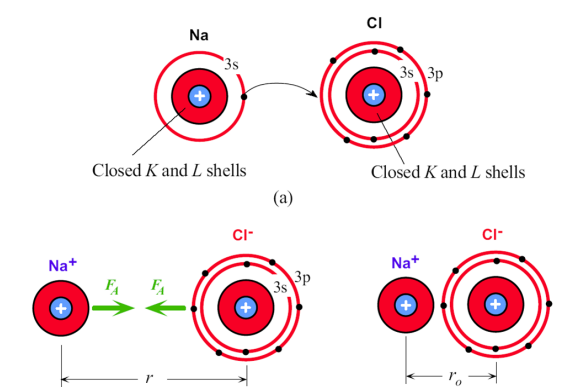
\includegraphics[width=\linewidth]{Bilder/Ionenbindung}
	\end{minipage}
	\hfill
	\begin{minipage}{0.48\linewidth}
		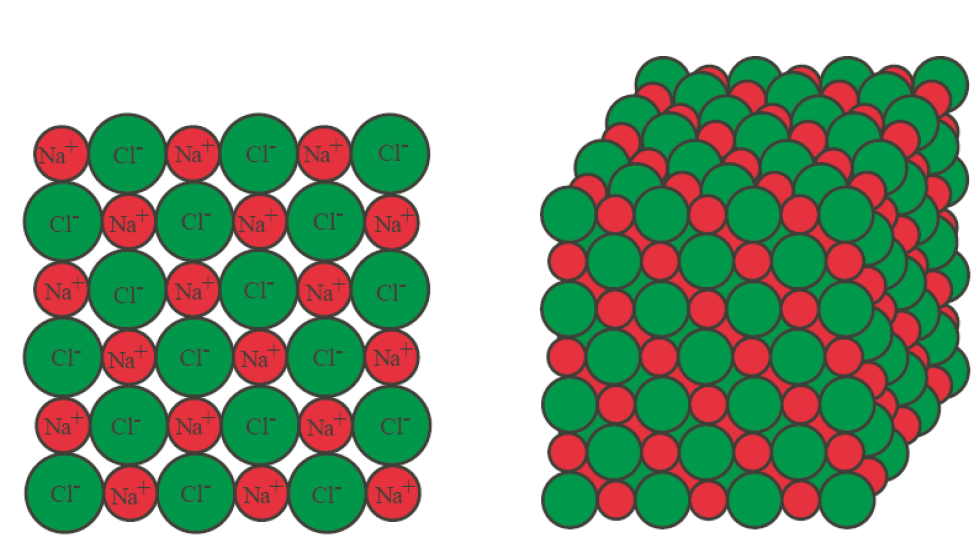
\includegraphics[width=\linewidth]{Bilder/Ionenbindung_2}
	\end{minipage}\vspace{1em}
	\begin{itemize}
		\item \textbf{wenig Valenzelektronen} (Atom A) \& \textbf{viele Valenzelektronen} (Atom B) $\to$ Elektron wird von A zu B übertragen (Bildung von Ionen)
		\item Anziehung durch Coulombkraft
		\item NaCl: bekanntes Beispiel
	\end{itemize}\vspace{1em}
	
	Ionisierungsenergie mittels modifiziertem Lennard-Jones-Potential:
	
	$$E_{tot} = -\frac{M\cdot e^2}{4\pi \varepsilon_0 r_0} + \frac{B}{r^m_0} + E_{\text{ion}} \quad M = 1.748 \,  (\text{Mandelung-Konstante})$$

\subsubsection{Wasserstoffbrücken und Van-der-Waals-Bindung}
	\begin{minipage}{0.45\linewidth}
		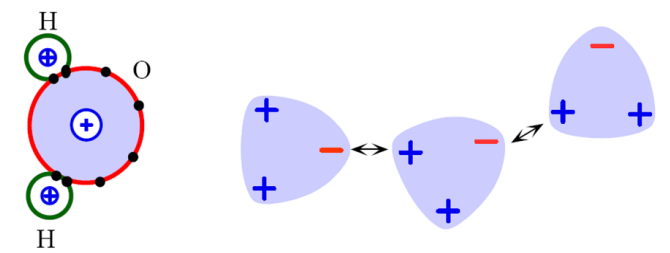
\includegraphics[width=0.99\linewidth]{Bilder/Wasserstoffbrücken}
	\end{minipage}
	\hfill
	\begin{minipage}{0.55\linewidth}
		\begin{itemize}
			\item Bsp. $H_2O$: kovalent, aber Elektronen stärker zu Sauerstoff gezogen $\to$ \textbf{polar}
			\item Polare Moleküle $\to$ Dipol-Dipol-Wechselwirkung (van-der-Waals)
			\item ist ein H-Atom involviert $\to$ \textbf{Wasserstoffbrücke}
			\item Dipolmoment kann aufgrund Flukt. ausgelöst werden $\to$ sehr schwache Bindung (Edelgase)
		\end{itemize}
	\end{minipage}

\subsubsection{Zusammenfassung}
\resizebox*{\columnwidth}{!}{
	\small
	\setlength{\tabcolsep}{2pt}
    \begin{tabular}{l l c c c c l}
        \toprule
        \textbf{Bond Type} & \textbf{Typical Solids} & \textbf{Bond Energy} & \textbf{Melt. Temp.} & \textbf{Elastic Mod.} & \textbf{Density} & \textbf{Typical} \\
        & & \textbf{(eV/atom)} & \textbf{($^\circ$C)} & \textbf{(GPa)} & \textbf{(g cm$^{-3}$)} & \textbf{Properties} \\
        \midrule
        Ionic & NaCl (rock salt) & 3.2 & 801 & 40 & 2.17 & Electrical insulators \\
              & & & & & & Conductive at high temp. \\
              & MgO (magnesia) & 10 & 2852 & 250 & 3.58 & High elastic modulus \\
              & & & & & & Hard, brittle, cleavable \\
        \midrule
        Metallic & Cu & 3.1 & 1083 & 120 & 8.96 & Electrical conductor \\
                 & & & & & & Good thermal conduction \\
                 & Mg & 1.1 & 650 & 44 & 1.74 & High elastic modulus \\
                 & & & & & & Ductile and shapable \\
        \midrule
        Covalent & Si & 4 & 1410 & 190 & 2.33 & Large elastic modulus \\
                 & & & & & & Hard and brittle \\
                 & C (diamond) & 7.4 & 3550 & 827 & 3.52 & Diamond: hardest material \\
                 & & & & & & High thermal conductivity \\
        \midrule
        van der Waals: & PVC (polymer) & --- & 212 & 4 & 1.3 & Low elastic modulus \\
        hydrogen bond & H$_2$O (ice) & 0.52 & 0 & 9.1 & 0.917 & Electrical insulator \\
                      & & & & & & Poor thermal conductivity \\
        \midrule
        van der Waals: & Crystalline & \multirow{2}{*}{0.09} & \multirow{2}{*}{$-189$} & \multirow{2}{*}{8} & \multirow{2}{*}{1.8} & Low elastic modulus \\
        induced dipole & argon & & & & & Electrical insulator \\
                       & & & & & & Large thermal expansion \\
        \bottomrule		
    \end{tabular}
	\setlength{\tabcolsep}{6pt}
}

\subsection{Kristallgitter und -strukturen}
	\begin{itemize}
		\item kristalline Körper haben periodische Anordnung
		\item Alle Kristalle bestehen aus:
		\begin{itemize}
			\item Gitter $\to$ gibt Periode an
			\item Basis $\to$ Atome mit örtlichem Versatz rel. zu jedem Gitterpunkt
		\end{itemize}
	\end{itemize}

\subsubsection{Triviale Basis}

\begin{minipage}{0.5\linewidth}
	\vspace{0.1mm}
	\centering
	\textbf{Kubisch Flächenzentriert, fcc}

	(auch dichtest-gepackte Gitterstruktur)

	(z.B. Kupferkristall)

	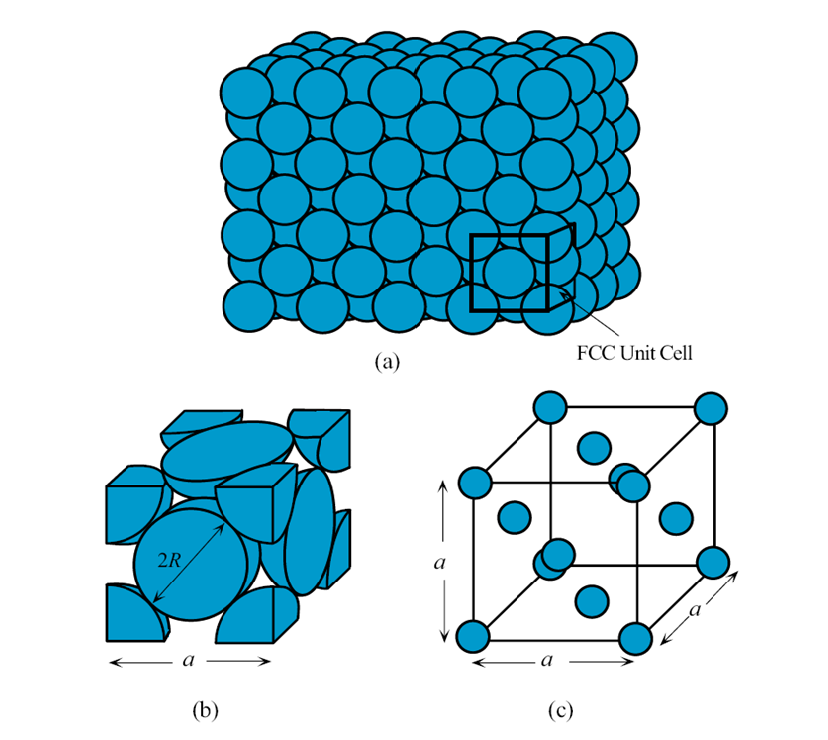
\includegraphics[width=0.9\linewidth]{Bilder/flächenzentriert.png}
\end{minipage}
\hfill
\begin{minipage}{0.5\linewidth}
	\centering
	\textbf{Kubisch Raumzentriert, bcc}

	(z.B. Li, Na, Cr, Mo, W)

	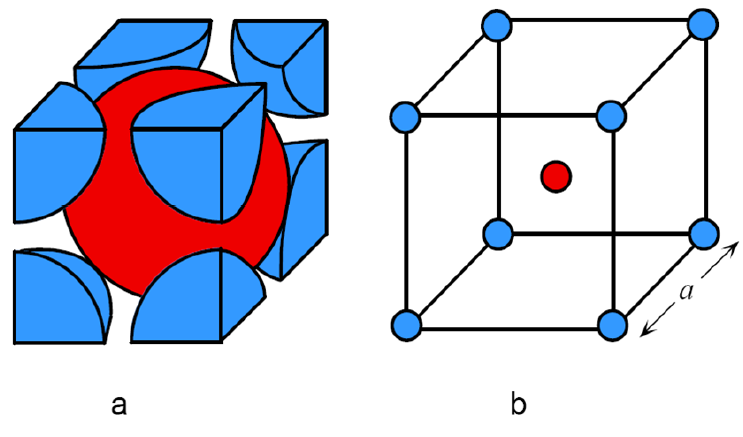
\includegraphics[width=0.9\linewidth]{Bilder/raumzentriert.png}

	\textbf{Hexagonal, hcp}

	(Be, Mg, Co, Zn, Zr, Cd)

	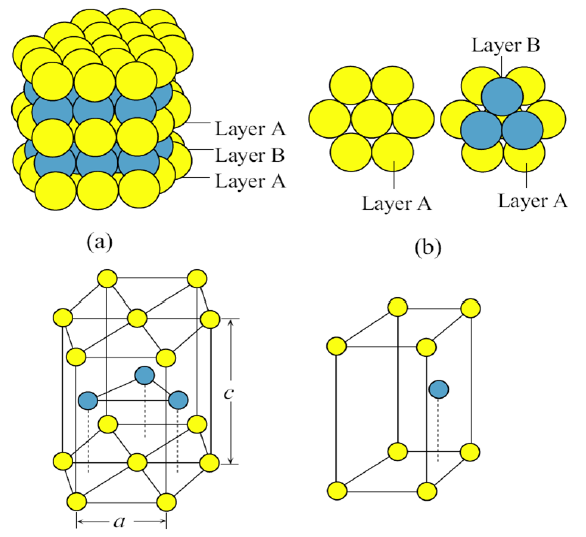
\includegraphics[width=0.9\linewidth]{Bilder/hexagonal.png}
\end{minipage}

\subsubsection{Nicht-triviale Basis}
\begin{minipage}{0.5\linewidth}
	\vspace{0.1mm}
	\centering
	\textbf{Diamant-Strukt., z.B. Si, Ge}

	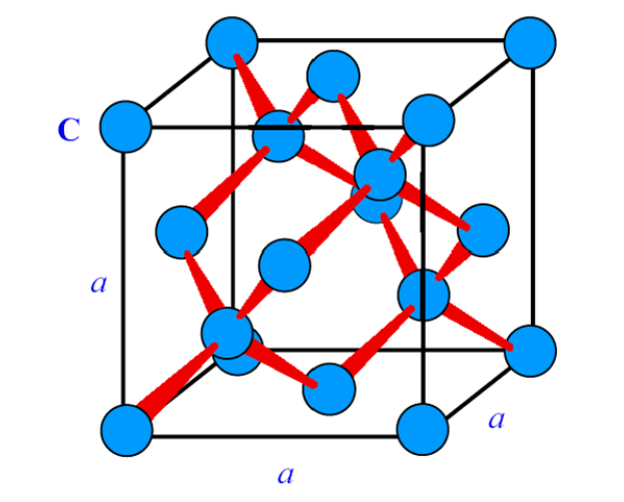
\includegraphics[width=0.9\linewidth]{Bilder/diamant-1-4.png}
\end{minipage}
\hfill
\begin{minipage}{0.5\linewidth}
	\centering
	\textbf{Zinkblende, z.B. ZnS, GaP, ZnTe, ...}

	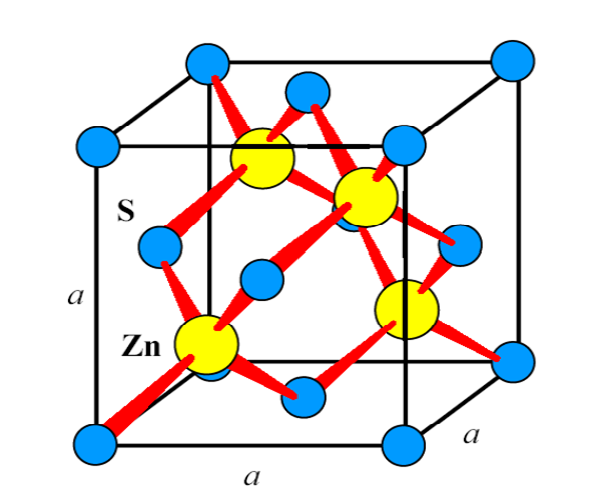
\includegraphics[width=0.85\linewidth]{Bilder/zinkblende.png}
\end{minipage}

\begin{tabular}{|l|l|c|}
\hline
\textbf{Categoria} & \textbf{Struttura} & \textbf{Atomi per Cella ($n$)} \\ \hline
\multirow{3}{*}{Triviale Basis} & Kubisch Flächenzentriert (fcc) & 4 \\ \cline{2-3} 
 & Kubisch Raumzentriert (bcc) & 2 \\ \cline{2-3} 
 & Hexagonal (hcp) & 6 \\ \hline
\multirow{2}{*}{Nicht-triviale Basis} & Diamant-Struktur & 8 \\ \cline{2-3} 
 & Zinkblende & 4 + 4 \\ \hline
\end{tabular}

\subsubsection{Gitterkonstante (z.B. für bcc-Kristalle)}
Grundsatz: Würfeldiagonale in Radien der Atome ausdrücken

$ \underbrace{\sqrt{3a^2}}_{\text{Würfeldiagonale}} = \underbrace{4 \cdot R}_{\text{Raggio atomico}} 
\quad \Leftrightarrow a = \frac{4R}{\sqrt{3}} \qquad \Rightarrow 
\quad (a) = \text{Gitterkonstante} $


% --- Densità ---
\subsubsection{Densità del materiale ($\rho$)}

La densità è il rapporto tra la massa totale degli atomi nella cella e il volume della cella stessa:

\begin{minipage}{0.4\columnwidth}
	$$\rho = \frac{n \cdot M}{a^3 \cdot N_A}$$
\end{minipage}
\begin{minipage}{0.6\columnwidth}
	\begin{itemize}
		\item $n$: Numero atomi per cella unitaria.
		\item $M$: Massa atomica $[\frac{\kilogram}{\mole}]$.
		\item $a$: Gitterkostanten
		\item $N_A \approx 6.022 \times 10^{23} \, \text{mol}^{-1}$ (Costante di Avogadro).
	\end{itemize}
\end{minipage}

% --- Concentrazione Atomica ---
\subsubsection{Concentrazione Atomica ($n_{at}$)}

Numero di atomi per unità di volume:

\begin{minipage}{0.4\columnwidth}
	$$n_{at} = \frac{n}{V_{cella}} = \frac{n}{a^3}$$
\end{minipage}
\begin{minipage}{0.6\columnwidth}
	\begin{itemize}
		\item $n$: Numero atomi per cella unitaria.
	\end{itemize}
\end{minipage}

% --- Fattore di Riempimento ---
\subsubsection{Packungsdichte ($P$ o Füllfaktor)}

Frazione di volume occupata dagli atomi (sfere rigide):

$$P = \frac{n \cdot V_{atomo}}{V_{cella}} = \frac{n \cdot \frac{4}{3}\pi R^3}{a^3}$$


% --- Densità Gas di Elettroni ---
\subsubsection{Densità del gas di elettroni liberi ($n_e$)}
Numero di elettroni di conduzione per unità di volume:

$$n_e = Z \cdot n_{at}$$

Dove $Z$ è il numero di elettroni ceduti da ogni singolo atomo al "gas".

% Bravais-Gitter (alle 14) wurden hier nicht inkludiert, Platzverschwendung, siehe Vorl Kap1